\section[Atributos de Requisitos]{Atributos de Requisitos}

%De acordo com o \citeonline{openUp}, atributos dos Requisitos são as propriedades de um requisito. Assim como uma entidade qualquer no contexto de desenvolvimento de software possui seus atributos, um requisito também possui os seus. 
%
%De maneira semelhante a uma entidade do tipo pessoa que possui atributos, tais como idade, cor do cabelo e sexo, cada requisito possui uma origem, uma importância relativa e a data em que foi criado, por exemplo. \cite{openUpBasic}.
%
%De acordo com o \citeonline{openUpBasic}, os atributos são uma fonte muito importante de informações sobre os requisitos e têm a intenção de capturar informações adicionais de cada requisito. Além de apenas definir as propriedades de um requisito, se bem definidos, os atributos podem fornecer significantes informações sobre o estado do desenvolvimento de um sistema. Estabelecendo um paralelo com uma consulta em um banco de dados em que se deseja encontrar todos os homens com cabelo castanho e idade maior que 30 anos, é possível consultar os 
%atributos de um requisito para encontrar os requisitos de alta prioridade para o cliente nos últimos 30 dias. 
%\cite{openUpBasic}.

\subsection{Descrição}

Com o objetivo de acompanhar e gerir da melhor maneira possível os requisitos, foram estabelecidos os seguintes atributos de requisitos:
\begin{itemize}
\item Data de entrega:
Data em que o requisito deve ser fornecido. Os valores deste atributo serão as próprias datas planejadas de entrega do requisito.

\begin{table}[h]
\centering
\caption{Descrição dos valores do atributo Data de entrega}
\label{Rotulo}
\begin{tabular}{|l|l|}
\hline
\textbf{Valor} & \textbf{Descrição} \\
\hline
Data & Data planejada para entrega do requisito. \\ \hline
\end{tabular}
\end{table}

%Esse atributo foi definido por fornecer de maneira rápida a previsão de entrega do requisito. Dessa maneira, permite uma visão ampla do planejamento de requisitos, auxiliando nas ações de gerenciamento dos requisitos.
\item Dificuldade:
Uma indicação do nível de esforço necessário ou quão difícil será implementar o requisito. Este atributo pode assumir os valores: alta, média ou baixa.

\begin{table}[h]
\centering
\caption{Descrição dos valores do atributo Dificuldade}
\label{Rotulo}
\begin{tabular}{ | l | p{0.8\linewidth} | }
\hline
\textbf{Valor} & \textbf{Descrição} \\ \hline
Alta  &  Requisito com implementação complexa, em função de: dificultadores técnicos, alterarem a implementação de muitos requisitos e/ou que tenham relacionamento com sistemas externos. \\ \hline
Média & Requisito com implementação não trivial, poucos dificultadores técnicos, alterarem a implementação de poucos requisitos e sem relação com sistemas externos. \\ \hline
Baixa & Requisito com uma implementação trivial, sem: dificultadores técnicos, alterações na implementação de outros requisitos ou relação com outros sistemas externos. \\ \hline
\end{tabular}
\end{table}

%Esse atributo foi escolhido em razão de informar o quão difícil será implementar um requisito, fornecendo dados que auxiliam no planejamento e organização dos esforços para conclusão das atividades de desenvolvimento de requisitos e para alcançar os resultados esperados.

\item Status:
Grau de completude, ou seja, o progresso da implementação de um requisito. Este atributo pode adquirir os seguintes valores: completo, parcialmente concluído ou não Iniciado.

\begin{table}[h]
\centering
\caption{Descrição dos valores do atributo Status}
\label{Rotulo}
\begin{tabular}{ | l | p{0.5\linewidth} | }
\hline
\textbf{Valor} & \textbf{Descrição} \\ \hline
100\% &  Indica que o requisito foi completamente implementado. \\ \hline
50\% & Indica que o requisito foi parcialmente implementado e ainda está sendo implementado. \\ \hline
0\% & Indica que o requisito ainda não começou a ser implementado. \\ \hline
\end{tabular}
\end{table}

%Esse atributo foi definido com o intuito de fornecer, a qualquer momento do desenvolvimento dos requisitos, a situação atual do requisito, em relação ao andamento de sua implementação. Ele permite que se tenha uma visão total do andamento do projeto, a partir de cada requisito.

\item Prioridade:
Declaração da importância relativa do requisito para os \textit{Stakeholders} (envolvidos ou interessados no desenvolvimento do software). Pode receber os seguintes valores: alta, média ou baixa.

\begin{table}[h]
\centering
\caption{Descrição dos valores do atributo Prioridade. Fonte: \cite{atributos}(Adaptado)   }
\label{Rotulo}
\begin{tabular}{ | l | p{0.8\linewidth} | }
\hline
\textbf{Valor} & \textbf{Descrição} \\ \hline
Alta &  Requisitos imprescindíveis. O fracasso em sua implementação indica que o sistema não irá atender às necessidades dos interessados. São requisitos fundamentais para o sucesso do projeto. \\ \hline
Média & Requisitos importantes para a eficácia ou eficiência do sistema. Sua não implementação afeta a satisfação do usuário e/ou o valor agregado do produto e o não atendimento não determina o fracasso do projeto. \\ \hline
Baixa & Requisitos úteis, porém menos críticos, sendo usados menos frequentemente. Não possui muito significado para a satisfação do usuário e seu atendimento pode ser postergado. \\ \hline
\end{tabular}
\end{table}

%\normalsize Esse atributo foi escolhido em razão de identificar o quão importante um requisito é para os envolvidos no projeto. Ele permite priorizar e planejar a implementação dos requisitos de acordo com suas prioridades, priorizando os requisitos de prioridade mais alta.


\end{itemize}

\subsection{Aplicação}

A partir da definição dos atributos, eles foram aplicados às \textit{Features} e às Histórias de Usuários, não sendo aplicados aos Épicos e ao Tema de Investimento por serem níveis de Requisitos muito elevados, com pouco grau de detalhamento, o que não agregaria valor ao projeto.

A ferramenta utilizada, \textit{TraceCloud}\footnotemark, além das informações de ID (\textit{Name}), Descrição (\textit{Description}) e 
Proprietário (\textit{Owner}) de um requisito, tem por padrão os atributos de Prioridade (\textit{Priority}) e Realizado (\textit{Percent Complet}),
que informa a porcentagem do quanto já foi realizado de um requisito. Com base nisso e nos quatro atributos definidos, optamos por utilizar
os dois atributos já providos pela ferramenta, e customizamos os outros dois, Dificuldade e Data de Entrega, para adequá-la ao que já 
havia sido proposto. 

\footnotetext{https://www.tracecloud.com/GloreeJava2/jsp/WebSite/TCHome.jsp}

A figura \ref{fig:atri_features} mostra os atributos aplicados às \textit{Features} e a tabela \ref{tab:atri_historias} exibe os atributos aplicados à todas as Histórias de Usuários, respectivamente. Já a figura \ref{fig:iteracao_atributos} mostra os atributos designados apenas as histórias implementadas na primeira iteração. Todo o conteúdo foi gerado pela ferramenta.

\begin{figure}[h]
 \centering
 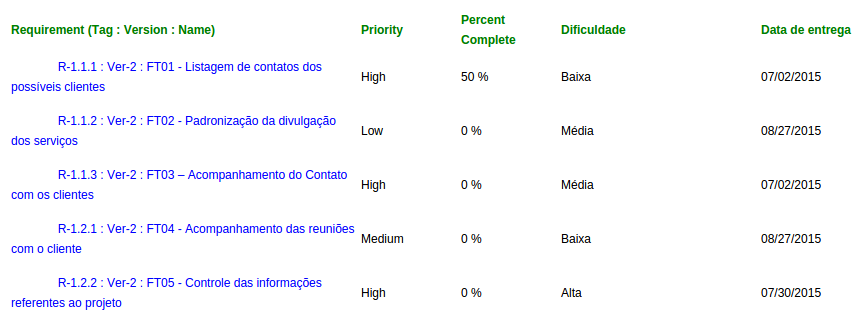
\includegraphics[width=1\linewidth]{figuras/atributos_features.png}
 \caption{Atributos aplicados às \textit{Features}}
 \label{fig:atri_features}
\end{figure}

\begin{table}
\centering
\caption{Atributos aplicados às Histórias de Usuários}
\label{tab:atri_historias}
\begin{tabular}{ | l | l | l | c | c | c |}
\hline
 ID  & Prioridade & Status & Dificuldade & Data de entrega \\ \hline
 US-01 & Alta     & 50               & Baixa       & 06/25/2015      \\\hline
 US-02 & Alta     & 50               & Baixa       & 06/25/2015      \\\hline
 US-03 & Média   & 0                & Média       & 07/02/2015      \\\hline
 US-04 & Média   & 0                & Baixa       & 07/02/2015      \\\hline
 US-05 & Média   & 50               & Média       & 06/25/2015      \\\hline
 US-06 & Alta     & 0                & Baixa       &                 \\\hline
 US-07 & Baixa      & 0                & Baixa       &                 \\\hline
 US-08 & Baixa      & 0                & Baixa       &                 \\\hline
 US-09 & Média   & 0                & Baixa       &                 \\\hline
 US-10 & Baixa      & 0                & Baixa       &                 \\\hline
 US-11 & Baixa      & 0                & Baixa       &                 \\\hline
 US-12 & Média   & 0                & Média       &                 \\\hline
 US-13 & Média   & 0                & Baixa       &                 \\\hline
 US-14 & Baixa      & 0                & Alta        &                 \\\hline
 US-16 & Baixa      & 0                & Média       &                 \\\hline
 US-17 & Baixa      & 0                & Baixa       &                 \\\hline
 US-18 & Alta     & 0                & Baixa       &                 \\\hline
 US-19 & Alta     & 0                & Baixa       &                 \\\hline
 US-20 & Alta     & 0                & Média       &                 \\\hline
 US-21 & Alta     & 0                & Baixa       &                 \\\hline
 US-22 & Alta     & 0                & Baixa       &                 \\\hline
 US-23 & Média   & 0                & Baixa       &                 \\\hline
 US-24 & Média   & 0                & Baixa       &                 \\\hline
 US-25 & Média   & 0                & Baixa       &                 \\\hline
 US-26 & Baixa      & 0                & Baixa       &                 \\\hline
 US-27 & Média   & 0                & Baixa       &                 \\\hline
 US-15 & Alta     & 0                & Baixa       &                 \\\hline
 US-28 & Média   & 0                & Baixa       &                 \\\hline
 US-29 & Baixa      & 0                & Baixa       &                 \\\hline
 US-30 & Média   & 0                & Baixa       &                 \\\hline
 US-31 & Baixa      & 0                & Baixa       &                 \\\hline
 US-32 & Média   & 0                & Baixa       &                 \\\hline
 US-33 & Média   & 0                & Média       &                 \\\hline
 US-34 & Média   & 0                & Baixa       &                 \\\hline
 US-35 & Baixa      & 0                & Baixa       &                 \\\hline
 US-36 & Média   & 0                & Baixa       &                 \\\hline
 US-37 & Baixa      & 0                & Baixa       &                 \\\hline
 US-38 & Média   & 0                & Baixa       &                 \\\hline
 US-40 & Média   & 0                & Média       &                 \\\hline
 US-39 & Média   & 0                & Baixa       &                 \\\hline
\end{tabular}
\end{table}

\begin{figure}[h]
\centering
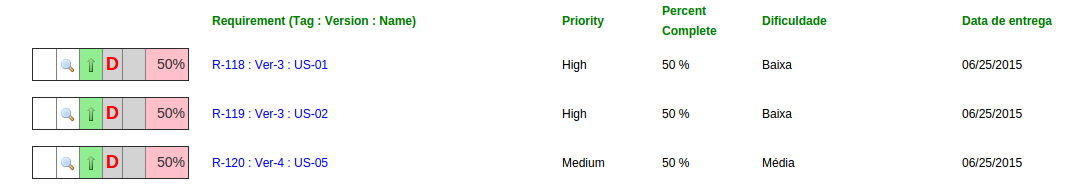
\includegraphics[width=1\linewidth]{figuras/iteracao_atributos.png}
\caption{Histórias de Usuários da primeira iteração com seus atributos}
\label{fig:iteracao_atributos}
\end{figure}
